\documentclass[portrait,final]{baposter}
%\documentclass[a4shrink,portrait,final]{baposter}
% Usa a4shrink for an a4 sized paper.

\tracingstats=2

\usepackage{times}
\usepackage{calc}
\usepackage{graphicx}
\usepackage{amsmath}
\usepackage{amssymb}
\usepackage{relsize}
\usepackage{multirow}
\usepackage{bm}

\usepackage{czech}
\usepackage[utf8]{inputenc}

\usepackage{graphicx}
\usepackage{multicol}

\usepackage{pgfbaselayers}
\pgfdeclarelayer{background}
\pgfdeclarelayer{foreground}
\pgfsetlayers{background,main,foreground}

\usepackage{helvet}
%\usepackage{bookman}
\usepackage{palatino}

\newcommand{\captionfont}{\footnotesize}

\selectcolormodel{cmyk}

\graphicspath{{images/}}

%%%%%%%%%%%%%%%%%%%%%%%%%%%%%%%%%%%%%%%%%%%%%%%%%%%%%%%%%%%%%%%%%%%%%%%%%%%%%%%%
%%%% Some math symbols used in the text
%%%%%%%%%%%%%%%%%%%%%%%%%%%%%%%%%%%%%%%%%%%%%%%%%%%%%%%%%%%%%%%%%%%%%%%%%%%%%%%%
% Format 
\newcommand*{\SET}[1]  {\ensuremath{\mathcal{#1}}}
\newcommand*{\MAT}[1]  {\ensuremath{\mathbf{#1}}}
\newcommand*{\VEC}[1]  {\ensuremath{\bm{#1}}}
\newcommand*{\CONST}[1]{\ensuremath{\mathit{#1}}}
\newcommand*{\norm}[1]{\mathopen\| #1 \mathclose\|}% use instead of $\|x\|$
\newcommand*{\abs}[1]{\mathopen| #1 \mathclose|}% use instead of $\|x\|$
\newcommand*{\absLR}[1]{\left| #1 \right|}% use instead of $\|x\|$

%%%%%%%%%%%%%%%%%%%%%%%%%%%%%%%%%%%%%%%%%%%%%%%%%%%%%%%%%%%%%%%%%%%%%%%%%%%%%%%%
% Multicol Settings
%%%%%%%%%%%%%%%%%%%%%%%%%%%%%%%%%%%%%%%%%%%%%%%%%%%%%%%%%%%%%%%%%%%%%%%%%%%%%%%%
\setlength{\columnsep}{0.7em}
\setlength{\columnseprule}{0mm}


%%%%%%%%%%%%%%%%%%%%%%%%%%%%%%%%%%%%%%%%%%%%%%%%%%%%%%%%%%%%%%%%%%%%%%%%%%%%%%%%
% Save space in lists. Use this after the opening of the list
%%%%%%%%%%%%%%%%%%%%%%%%%%%%%%%%%%%%%%%%%%%%%%%%%%%%%%%%%%%%%%%%%%%%%%%%%%%%%%%%
\newcommand{\compresslist}{%
\setlength{\itemsep}{1pt}%
\setlength{\parskip}{0pt}%
\setlength{\parsep}{0pt}%
}


%%%%%%%%%%%%%%%%%%%%%%%%%%%%%%%%%%%%%%%%%%%%%%%%%%%%%%%%%%%%%%%%%%%%%%%%%%%%%%
%%% Begin of Document
%%%%%%%%%%%%%%%%%%%%%%%%%%%%%%%%%%%%%%%%%%%%%%%%%%%%%%%%%%%%%%%%%%%%%%%%%%%%%%

\begin{document}

%%%%%%%%%%%%%%%%%%%%%%%%%%%%%%%%%%%%%%%%%%%%%%%%%%%%%%%%%%%%%%%%%%%%%%%%%%%%%%
%%% Here starts the poster
%%%---------------------------------------------------------------------------
%%% Format it to your taste with the options
%%%%%%%%%%%%%%%%%%%%%%%%%%%%%%%%%%%%%%%%%%%%%%%%%%%%%%%%%%%%%%%%%%%%%%%%%%%%%%
% Define some colors
\definecolor{silver}{cmyk}{0,0,0,0.3}
\definecolor{yellow}{cmyk}{0,0,0.9,0.0}
\definecolor{reddishyellow}{cmyk}{0,0.22,1.0,0.0}
\definecolor{black}{cmyk}{0,0,0.0,1.0}
\definecolor{darkYellow}{cmyk}{0,0,1.0,0.5}
\definecolor{darkSilver}{cmyk}{0,0,0,0.1}

\definecolor{lightyellow}{cmyk}{0,0,0.3,0.0}
\definecolor{lighteryellow}{cmyk}{0,0,0.1,0.0}
\definecolor{lighteryellow}{cmyk}{0,0,0.1,0.0}
\definecolor{lightestyellow}{cmyk}{0,0,0.05,0.0}

%%
\typeout{Poster Starts}
\background{
  \begin{tikzpicture}[remember picture,overlay]%
    \draw (current page.north west)+(-2em,2em) node[anchor=north west] {\includegraphics[height=1.1\textheight]{silhouettes_background}};
  \end{tikzpicture}%
}

\newlength{\leftimgwidth}
\begin{poster}%
  % Poster Options
  {
  % Show grid to help with alignment
  grid=no,
  % Column spacing
  colspacing=1em,
  % Color style
  bgColorOne=lighteryellow,
  bgColorTwo=lightestyellow,
  borderColor=reddishyellow,
  headerColorOne=yellow,
  headerColorTwo=reddishyellow,
  headerFontColor=black,
  boxColorOne=lightyellow,
  boxColorTwo=lighteryellow,
  % Format of textbox
  textborder=roundedleft,
%  textborder=rectangle,
  % Format of text header
  eyecatcher=no,
  headerborder=open,
  headerheight=0.08\textheight,
  headershape=roundedright,
  headershade=plain,
  headerfont=\Large\textsf, %Sans Serif
  boxshade=plain,
%  background=shade-tb,
  background=plain,
  linewidth=2pt
  }
  % Eye Catcher
  {} % No eye catcher for this poster. (eyecatcher=no above). If an eye catcher is present, the title is centered between eye-catcher and logo.
  % Title
  {\sf %Sans Serif 
  %\bf% Serif
  Laser pointer drawing}
  % Authors
  {\sf %Sans Serif
  % Serif
  \vspace{1em} Tomáš Pokorný (xtompok@gmail.com)
  }
  % University logo
  {% The makebox allows the title to flow into the logo, this is a hack because of the L shaped logo.
  }

  \tikzstyle{light shaded}=[top color=baposterBGtwo!30!white,bottom color=baposterBGone!30!white,shading=axis,shading angle=30]

  % Width of left inset image
     \setlength{\leftimgwidth}{0.78em+8.0em}

%%%%%%%%%%%%%%%%%%%%%%%%%%%%%%%%%%%%%%%%%%%%%%%%%%%%%%%%%%%%%%%%%%%%%%%%%%%%%%
%%% Now define the boxes that make up the poster
%%%---------------------------------------------------------------------------
%%% Each box has a name and can be placed absolutely or relatively.
%%% The only inconvenience is that you can only specify a relative position 
%%% towards an already declared box. So if you have a box attached to the 
%%% bottom, one to the top and a third one which should be in between, you 
%%% have to specify the top and bottom boxes before you specify the middle 
%%% box.
%%%%%%%%%%%%%%%%%%%%%%%%%%%%%%%%%%%%%%%%%%%%%%%%%%%%%%%%%%%%%%%%%%%%%%%%%%%%%%
    %
    % A coloured circle useful as a bullet with an adjustably strong filling
    \newcommand{\colouredcircle}[1]{%
      \tikz{\useasboundingbox (-0.2em,-0.32em) rectangle(0.2em,0.32em); \draw[draw=black,fill=baposterBGone!80!black!#1!white,line width=0.03em] (0,0) circle(0.18em);}}

%%%%%%%%%%%%%%%%%%%%%%%%%%%%%%%%%%%%%%%%%%%%%%%%%%%%%%%%%%%%%%%%%%%%%%%%%%%%%%
  \headerbox{Abstract}{name=abstract,column=0,row=0,span=3}{
%%%%%%%%%%%%%%%%%%%%%%%%%%%%%%%%%%%%%%%%%%%%%%%%%%%%%%%%%%%%%%%%%%%%%%%%%%%%%%
   {}Project Laser pointer drawing is about computer processing images captured through the webcam. In image from camera is found lighted point, coordinates of this point are transformed to dataprojector coordinates and they are used to draw on screen or do something else. Application is written in Objective C and uses Mac OS X libraries.  \vspace{0.3em}
 }

%%%%%%%%%%%%%%%%%%%%%%%%%%%%%%%%%%%%%%%%%%%%%%%%%%%%%%%%%%%%%%%%%%%%%%%%%%%%%%
  \headerbox{Equipment}{name=equipment,column=0,below=abstract}{
%%%%%%%%%%%%%%%%%%%%%%%%%%%%%%%%%%%%%%%%%%%%%%%%%%%%%%%%%%%%%%%%%%%%%%%%%%%%%%
This equipment is needed to run the project:
\begin{itemize}
 \item Mac
 \item webcam
 \item dataprojector
 \item laser pointer
\end{itemize}
The project uses CocoaSequenceGrabber for getting images from camera, so it works best with the integrated iSight. Working with externals camera is not tested. Used resolution of the camera is $320 \times 240$. Recommended Mac has 2 GHz processor to process images fast enough. Used resolution of dataprojector is $800 \times 600$ and the color of the laser pointer is red.
}

%%%%%%%%%%%%%%%%%%%%%%%%%%%%%%%%%%%%%%%%%%%%%%%%%%%%%%%%%%%%%%%%%%%%%%%%%%%%%%
  \headerbox{Processing image}{name=process,column=0,below=equipment}{
%%%%%%%%%%%%%%%%%%%%%%%%%%%%%%%%%%%%%%%%%%%%%%%%%%%%%%%%%%%%%%%%%%%%%%%%%%%%%%
Images are captured by framework CocoaSequenceGrabber. We need to find the lighted point, if it is on image. To find it, it is used cross method. In this method there are three types of points:\\
\begin{center}
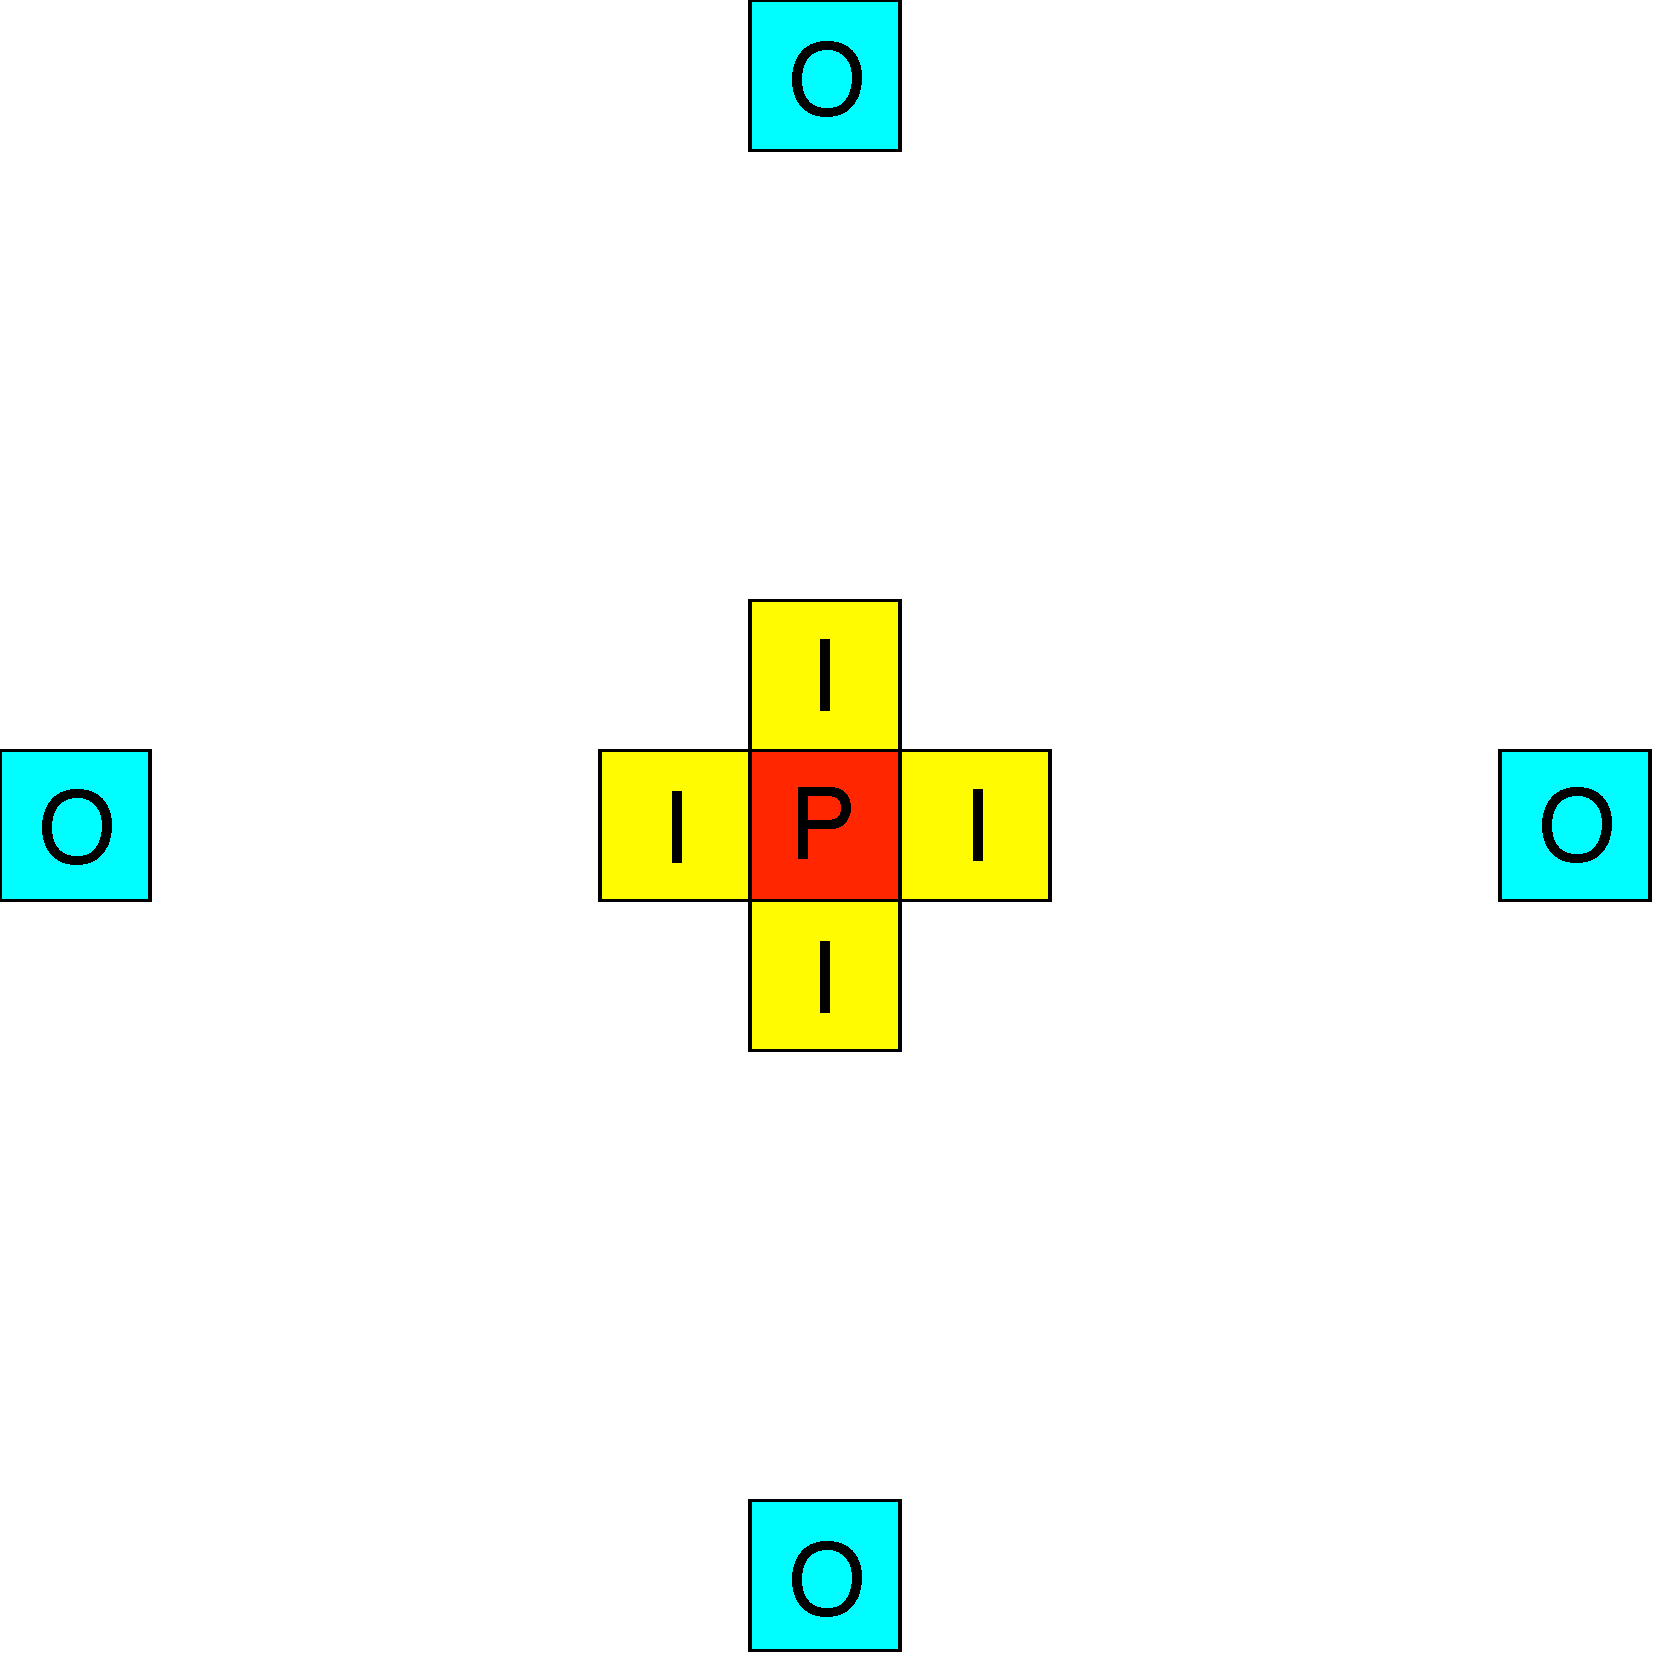
\includegraphics[scale=.2]{../CrossImageProcess.pdf}\\
\end{center}
\begin{itemize}
 \item Central point $P$, which is the current tested point
 \item Inner points $I$, whose are on the top, bottom left and right of the central point.
 \item Outer points $O$, whose are five pixels on the top, bottom, left and right of the central point and represents the background
\end{itemize}
The central point goes point by point through all image and computes average of inner and outer points, whose are aviable and compare them with configured values. If it's lower than in configuration, they are discarted. From not discarted points is chosen point with maximal values.

\vspace{0.3em}
  }

%%%%%%%%%%%%%%%%%%%%%%%%%%%%%%%%%%%%%%%%%%%%%%%%%%%%%%%%%%%%%%%%%%%%%%%%%%%%%%
  \headerbox{Transformation}{name=transformation,column=1,below=abstract}{
%%%%%%%%%%%%%%%%%%%%%%%%%%%%%%%%%%%%%%%%%%%%%%%%%%%%%%%%%%%%%%%%%%%%%%%%%%%%%%
We need to transform coordinates from image to projector, because the axis of the camera isn't parallel with axis of the screen, so the image is distorted -- the screen is not rectangle on the image from camera, but some quadrilateral.
%%%% DOPLNIT OBRÁZEK %%%%%%
To transform it to rectangle is used perspective transformation, where each point is transformed with these equations:  

\begin{align}
x'&=\frac{a_0x+a_1y+a_2}{a_6x+a_7y+1}\\ 
 y'&=\frac{a_3x+a_4y+a_5}{a_6x+a_7y+1} 
\end{align}
The transformation could be written to matrix:
$$
\left[ \begin{array}{c}
u \\
v \\
w \end{array} \right]
=
\left[ \begin{array}{c}
x \\
y \\
1 \end{array} \right]
\cdot
\left[ \begin{array}{ccc}
a_0 & a_1 & a_2 \\
a_3 & a_4 & a_5 \\
a_6 & a_7 & 1 \end{array} \right]
$$
To get transformed values of $x$ and $y$ we need to normalise them:
\begin{eqnarray*}
 x' &=& \frac{u}{w}\\
 y' &=& \frac{v}{w}\\
\end{eqnarray*}
  \vspace{0.5em}
  }

%%%%%%%%%%%%%%%%%%%%%%%%%%%%%%%%%%%%%%%%%%%%%%%%%%%%%%%%%%%%%%%%%%%%%%%%%%%%%%
  \headerbox{Calibration}{name=calibration,column=1,below=transformation}{
%%%%%%%%%%%%%%%%%%%%%%%%%%%%%%%%%%%%%%%%%%%%%%%%%%%%%%%%%%%%%%%%%%%%%%%%%%%%%%
  To get the right values of $a_0, \dots, a_7$ we need some calibration points. For this reason, there is an calibration. After start of calibration, four calibration points are showed in sequence by dataprojector in corners of drawable area.
  \begin{center}
  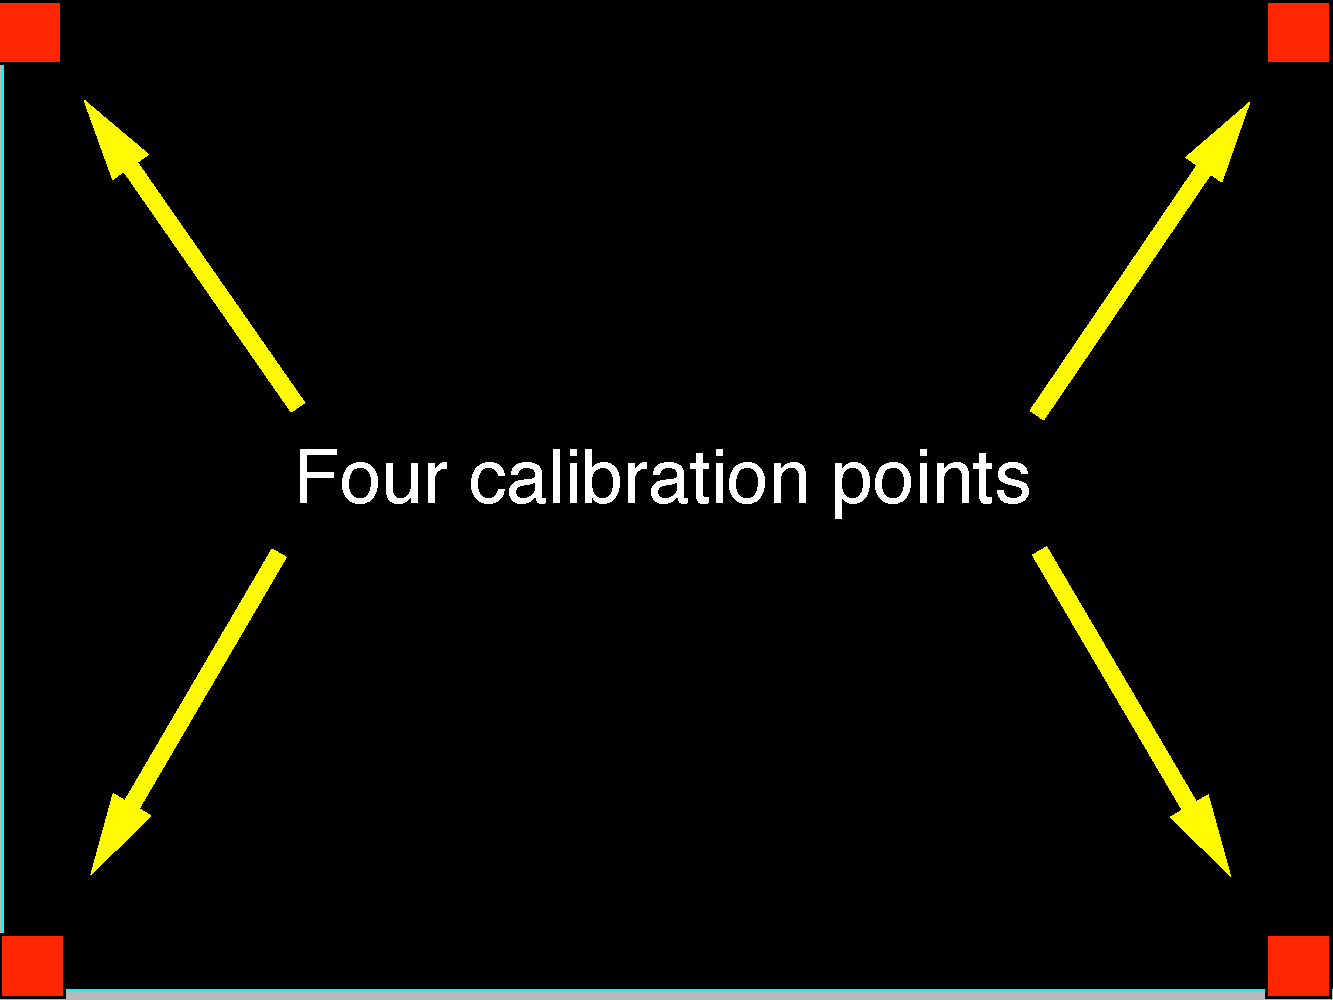
\includegraphics[scale=.3]{../Calibration_image.pdf}
  \end{center}
  \vspace{0.3em}
 For each point program finds its position in image using cross method from Processing image. After all points are showed, coordinates of their positions are sent to transformation classes, which computes its constants for transformation. 
  }

%%%%%%%%%%%%%%%%%%%%%%%%%%%%%%%%%%%%%%%%%%%%%%%%%%%%%%%%%%%%%%%%%%%%%%%%%%%%%%
  \headerbox{Viewing}{name=viewing,column=2,below=abstract}{
%%%%%%%%%%%%%%%%%%%%%%%%%%%%%%%%%%%%%%%%%%%%%%%%%%%%%%%%%%%%%%%%%%%%%%%%%%%%%%
  There are many possible ways how to visualise results, some of them are mentioned below.
  \vspace{0.3em}
  }

%%%%%%%%%%%%%%%%%%%%%%%%%%%%%%%%%%%%%%%%%%%%%%%%%%%%%%%%%%%%%%%%%%%%%%%%%%%%%%
  \headerbox{Single color drawing}{name=singlecol,column=2,below=viewing}{
%%%%%%%%%%%%%%%%%%%%%%%%%%%%%%%%%%%%%%%%%%%%%%%%%%%%%%%%%%%%%%%%%%%%%%%%%%%%%%
  On the current position of laser pointer is showed cross and the position is added to the \texttt{NSBezierPath} object which is drawed with green color. If there isn't a point from laser pointer, cross isn't drawed and the path is diconnected. If the light is back again, virtual "pen" is moved to new position and starts drawing again. The width of "pen" could be changed from GUI. From GUI could be also reseted a drawing.
  \vspace{0.3em}
  }

%%%%%%%%%%%%%%%%%%%%%%%%%%%%%%%%%%%%%%%%%%%%%%%%%%%%%%%%%%%%%%%%%%%%%%%%%%%%%%
  \headerbox{Multi color drawing}{name=multicol,column=2,below=singlecol}{
%%%%%%%%%%%%%%%%%%%%%%%%%%%%%%%%%%%%%%%%%%%%%%%%%%%%%%%%%%%%%%%%%%%%%%%%%%%%%%
  Principle of this drawing is the same as in single color drawing. There are some aditional things -- three squares with three colors. If the point from pointer is in this square, color of the virtual "pen" changes to the color of square.
  \begin{center}
  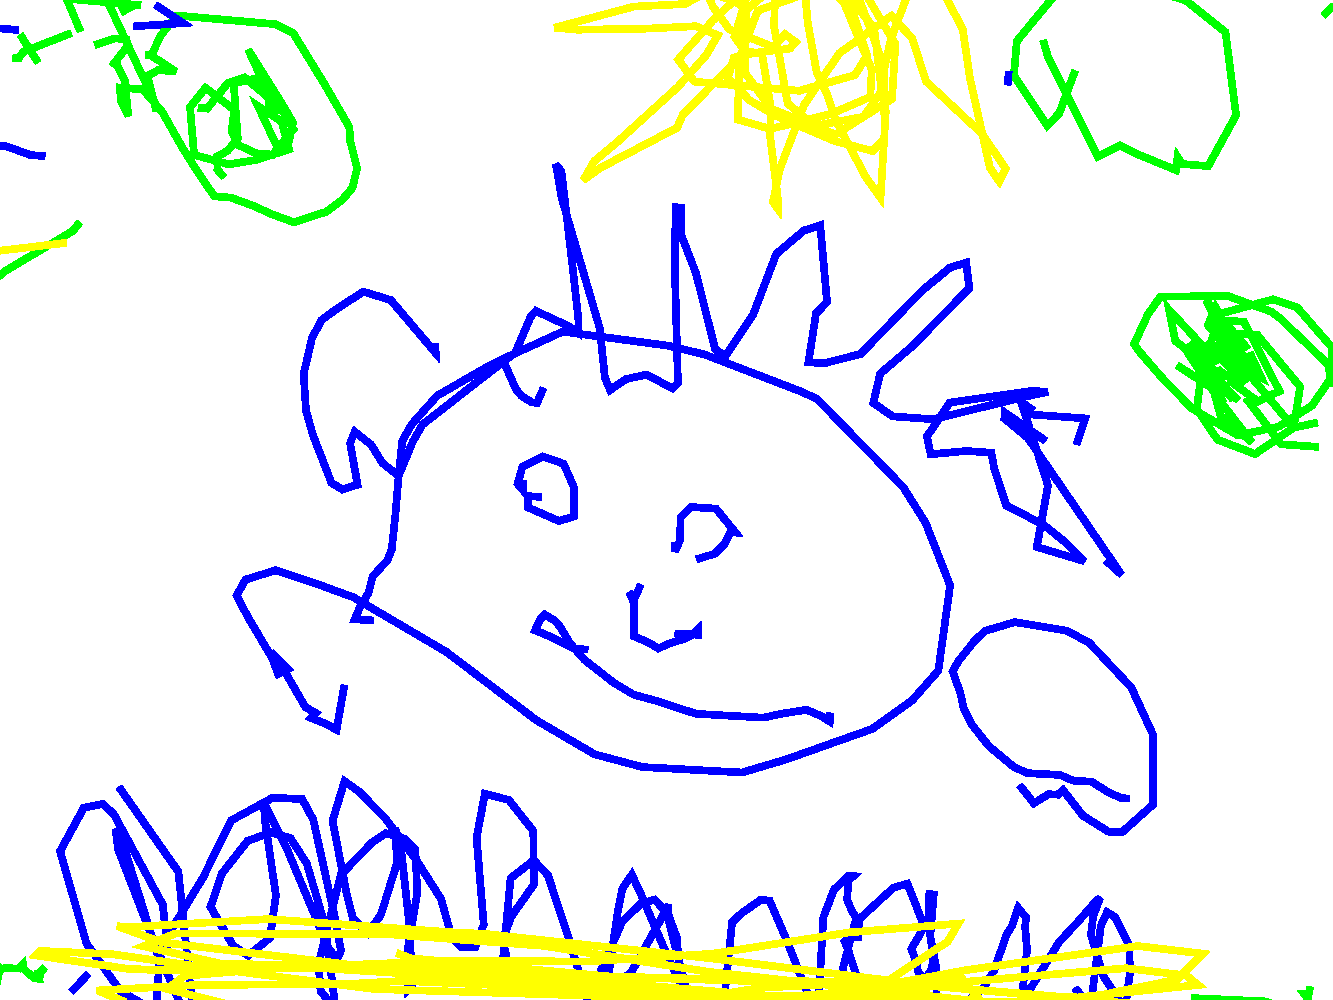
\includegraphics[scale=.2]{./xicht.pdf}
  \end{center}
  \vspace{0.3em}
  }

%%%%%%%%%%%%%%%%%%%%%%%%%%%%%%%%%%%%%%%%%%%%%%%%%%%%%%%%%%%%%%%%%%%%%%%%%%%%%%
  \headerbox{Shooting baloons}{name=baloons,column=2,below=multicol}{
%%%%%%%%%%%%%%%%%%%%%%%%%%%%%%%%%%%%%%%%%%%%%%%%%%%%%%%%%%%%%%%%%%%%%%%%%%%%%%
  This is future application, which will be probably developed in few weeks or months. There will be moving baloons represented by circles on the screen. there will be moving with variable speeds and player will try to shoot them with laser pointer. In more advanced version of this game there could be more lasers with different colors, one for each player.
  \vspace{0.3em}
  }

%%%%%%%%%%%%%%%%%%%%%%%%%%%%%%%%%%%%%%%%%%%%%%%%%%%%%%%%%%%%%%%%%%%%%%%%%%%%%%
  \headerbox{Thanks}{name=thanks,column=1,span=2,above=bottom}{
%%%%%%%%%%%%%%%%%%%%%%%%%%%%%%%%%%%%%%%%%%%%%%%%%%%%%%%%%%%%%%%%%%%%%%%%%%%%%%
  \smaller 
  Thanks to Marek Blaha, Tomáš Gavenčak, Lukáš Langer, Jan Olšina and other people, who helped me with the project.
  \hspace{1em}  }
%%%%%%%%%%%%%%%%%%%%%%%%%%%%%%%%%%%%%%%%%%%%%%%%%%%%%%%%%%%%%%%%%%%%%%%%%%%%%%
  \headerbox{References}{name=references,column=0,above=bottom}{
%%%%%%%%%%%%%%%%%%%%%%%%%%%%%%%%%%%%%%%%%%%%%%%%%%%%%%%%%%%%%%%%%%%%%%%%%%%%%%
    \smaller
    \vspace{-0.4em}
    \bibliographystyle{ieee}
    \renewcommand{\section}[2]{\vskip 0.05em}
      \begin{thebibliography}{1}\itemsep=-0.01em
      \setlength{\baselineskip}{0.4em}
      \bibitem{}
       D.-K.~Kim, B.-T. Jang, C.-J. Hwang
       \newblock {A} {P}lanar Perspective Image Matching using Point Correspondences and Rectangle-to-Quadrilateral Mapping
       \newblock in {\em Image Analysis and Interpretation, IEEE Southwest Symposium 2002}

      \end{thebibliography}
  }

\end{poster}%
\end{document}
